\chapter{Circuits RLC en sèrie}

\begin{resum}
abstract
\end{resum}

\section{Introducció}
En general, la intensitat que circula per un circuit RLC sotmès a una tensió \( V(t) \) està governada per la següent equació diferencial
\begin{equation} \label{eq:llei RLC}
	\frac{d^2 I}{dt^2} + \frac{R}{L} \frac{dI}{dt} + \frac{1}{LC}I = \frac{1}{L}\frac{dV}{dt},
\end{equation}
on \( R \) és la resistència, \( L \) és la inductància de la bobina i \( C \) la capacitat del condensador. Podem reescriure l'\cref{eq:llei RLC} per trobar la llei que obeeix la tensió que cau a la resistència, \( V_R \):
\begin{equation} \label{eq:llei VR}
	\frac{d^2V_R}{dt^2} + \frac{R}{L}\frac{dV_R}{dt} + \frac{1}{LC}V_R = \frac{R}{L}\frac{dV}{dt}.
\end{equation}
Similarment també podem obtenir la llei que governa la caiguda de tensió en la bobina
\begin{equation} \label{eq:llei VC}
	\frac{d^2V_C}{dt^2} + \frac{R}{L}\frac{dV_C}{dt} + \frac{1}{LC}V_C = \frac{1}{LC}V.
\end{equation}
Observem que totes aquestes equacions són les d'un osci\l.lador forçat. la solució general és la suma d'una solució particular, que rep el nom de terme estacionari, i una solució del sistema homogeni, que rep el nom de terme transitori. La forma del terme transitori depèn dels paràmetres del circuit. En concret depèn del valor del discriminant
\begin{equation*}
	\Delta = \frac{R^2}{L^2} - \frac{4}{LC}.
\end{equation*}
Si \( \Delta < 0 \) el circuit està infraamortit i tenim osci\l.lacions a freqüència 
\begin{equation} \label{eq:freq amortida}
 	\omega = \frac{1}{2}\sqrt{-\Delta} = \frac{1}{2}\sqrt{\frac{4}{LC} - \frac{R^2}{L^2}}. 
\end{equation}
Si \( \Delta > 0 \) aleshores diem que el circuit es troba sobreamortit i no tenim osci\l.lacions, només una caiguda exponencial. En el cas que \( \Delta = 0 \) parlem d'amortiment crític. La resistència que dóna lloca a amortiment crític rep el nom de resistència crítica i es pot calcular imposant \( \Delta = 0 \) i resulta
\begin{equation} \label{eq:resistencia critica}
	R_C = 2\sqrt{\frac{L}{C}}. 
\end{equation}

En tots tres casos, el terme transitori va multiplicat per un factor \( e^{-\lambda t} \) on \( \lambda = \frac{R}{2L} \) rep el nom de constant d'amortiment. Per tant decaurà de forma exponencial, raó per la qual rep el nom de transitori. A la primera part de la pràctica analitzem un circuit en el règim transitori ---i.e. abans de que el terme transitori pugui decaure significativament--- i comprovarem com varia l'amortiment del circuit en funció de \( R \).  

Un cas particularment rellevant és el d'un circuit forçat amb una tensió s'entrada sinusoidal. En aquestes condicions podem observar el fenòment de ressonància, que té lloc quan la tensió d'entrada osci\l.la a la freqüència característica del circuit, 
\begin{equation}\label{eq:freq ressonancia}
	\omega_0 = \frac{1}{\sqrt{LC}}.
\end{equation}
En aquestes condicions ---i en general quan la tensió subministrada osci\l.la sinusoidalment en el temps---, en el règim estacionari totes les magnituds del circuit osci\l.len a la freqüència subministrada \( \omega \). L'amplitud i la diferència de fase d'aquestes osci\l.lacions, però, depenen de \( \omega \). Concretament, per al cas de \( V_R \) es té que el desfasament \( \phi \) amb \( V \) compleix
\begin{equation} \label{eq:desfasament}
	\tan{\phi} = \frac{\frac{1}{C\omega} - L\omega}{R}
\end{equation}
i 
\begin{equation} \label{eq:guany}
	\abs{T_R(\omega)} = \frac{R}{\sqrt{R^2 + \left(L\omega - \frac{1}{C\omega}\right)^2}},
\end{equation}
on \( \abs{T_R(\omega)} \) s'anomena el guany ---\( T_R(\omega) \) és una quantitat complexa que també conté informació sobre el desfasament, però el seu mòdul és precisament el quocient de les amplituds---.

A la segona part de la pràctica analitzarem aquest fenomen en el cas particular de la tensió de la resistència, \( V_R \).   

\section{Mètode experimental}
\subsection{Règim transitori}
\begin{figure}[htb]
	\centering \small \sffamily
	\begin{circuitikz} \draw
	(0,0) to[sqV] (6,0) -- (6,3)
	to[L = \SI{33}{mH}] (4,3)
	to[C = \SI{330}{pF}] (2,3)
	to[vR] (0,3) -- (0,0)
	(2,3) -- (2,4)
	to[voltmeter, l = \( V_C \)] (4,4) -- (4,3)
	;
\end{circuitikz}

	\caption{Esquema del circuit utilitzat per a la primera part}
	\label{fig:esquema transitori}
\end{figure}

En aquesta part de la pràctica s'analitzarà el comportament d'un circuit RLC en el règim transitori. Sobre un circuit amb una bobina d'inductància \( L = \SI{33}{mH} \), una resistència de \( R = \SI{180}{\ohm} \) i un condensador de capacitat \( C  = \SI{330}{pF} \) s'aplicarà un senyal rectangular periòdic d'amplitud \SI{5}{V}. Amb aquests paràmetres podem determinar la resistència crítica \( R_C \) del circuit amb l'\cref{eq:resistencia critica}. El valor de \( R_C \) és \SI{2d4}{\ohm}, de manera que estem en condicions d'infraamortiment. Per a mesurar el període de les osci\l.lacions del voltatge al condensador, \( V_C \), ajustarem la freqüència del senyal rectangular de manera que un període d'aquesta coincideixi amb 10 osci\l.lacions de la tensió al condensador, que s'està mesurant amb un osci\l.loscopi. D'aquesta manera, el període del senyal és 10 vegades el període de les osci\l.lacions.

Per a mesurar la resistència crítica del sistema substituïm la resistència fixa per una de variable. Per a diferents valors de resistència observem comportament infraamortit i sobreamortit. La resistència que es troba a la frontera entre els dos comportaments és \( R_C \).  

\subsection{Règim estacionari}
\begin{figure}[htb]
	\centering \small \sffamily
	\begin{circuitikz} \draw
	(0,0) to[sV] (6,0) -- (6,3)
	to[L = \SI{22}{mH}] (4,3)
	to[C = \SI{15}{mF}] (2,3)
	to[R = \SI{270}{\ohm}] (0,3) -- (0,0)
	(0,3) -- (0,4)
	to[voltmeter, l = \( V_R \)] (2,4) -- (2,3)
	(0,4) -- (0,5.5)
	to[voltmeter, l = \( V \)] (6,5.5) -- (6,3)
	;
\end{circuitikz}

	\caption{Esquema del circuit utilitzat per a la primera part}
	\label{fig:esquema estacionari}
\end{figure}

Per aquesta segona part realitzem mesures sobre un circuit RLC amb capacitat \( C = \SI{15}{mF} \), inductància \( L = \SI{22}{mH} \) i resistència \( R = \SI{2700}{\ohm} \). Després repetirem el procediment amb una resistència de \SI{270}{\ohm}. El circuit estarà sotmès a un voltatge d'entrada \( V \) de freqüència \( \omega \), que es pot controlar a través d'una font. Es mesuraran \( V \) i \( V_r \) amb un osci\l.loscopi.  

En primer lloc es determinarà per a quina freqüència d'entrada el circuit es troba en ressonància ---és a dir, per a quina freqüència el desfasament entre \( V_R \) i \( V \) és nul--- i el valor obtingut es compararà amb el valor calculat per a \( \omega_0 \) segons l'\cref{eq:freq ressonancia}. 

També es determinaran les freqüències de tall, que són les que compleixen \( \abs{T_R(\omega)} = \frac{1}{\sqrt{2}} \). Les freqüències de tall, \( \omega_1 \) i \( \omega_2 \) es poden calcular a priori segons les equacions
\begin{equation} \label{eq:freqs de tall}
	\begin{aligned}
		\omega_1\omega_2 &= \omega_0^2 \\
		\omega_2 - \omega_1 &= \frac{R}{L},
	\end{aligned}
\end{equation}
i els resultats es compararan amb les mesures preses. 

\section{Resultats}
\subsection{Règim transitori}
El valor obtingut per a la freqüència del circuit a partir dels valors coneguts de \( L \), \( C \) i \( R \) i de l'\cref{eq:freq amortida} és \SI{3.03d5}{rad.s^{-1}}. Això dóna un valor per al període de \SI{2.07d-5}{s}. El valor mesurat del període és \data{2.3}{0.1d-5}{s}. Tenim doncs un percentatge d'error de $11\%$. De manera que, tot i que per incerteses els valors no siguin compatibles, són força propers.

Per la resistència crítica, el valor obtingut experimentalment és \data{1.28}{0.01d4}{\ohm}, i el valor obtingut amb l'\cref{eq:resistencia critica} és \SI{2e4}{\ohm}. De nou, el percentatge d'error val $36\%$, resultat no tan satisfactori. 

La mesura del període d'oscil·lació del sistema no és llavors del tot compatible amb el valor teòric. Tampoc ho és el de la resistència crítica. El motiu principal d'aquesta gran discrepància és que en els càlculs no s'han considerat resistències adicionals, a més de la resistència del potenciòmetre. Efectivament, si hom calcula, a partir del valor mesurat del període de l'\cref{eq:freq amortida}, la resistència total a la que està sotmès el circuit, suposant que la capacitat i inductància total es corresponen amb els valors nominals, es troba que la resistència total és d'uns \SI{8.6}{k\ohm}. Com que la mesura es va realitzar amb una resistència nominal de \SI{180}{\ohm}, això vol dir que les resistències desconegudes contribueixen al voltant de \SI{8.4}{k\ohm} a la resistència total. Això vol dir que la resistència crítica del circuit és en realitat de \( \SI{12.8}{k\ohm} + \SI{8.4}{k\ohm} = \SI{21.2}{k\ohm} \), que s'ajusten molt millor als \SI{20}{k\ohm} predits teòricament.  

A la \cref{fig:oscilacions} hi ha representats les tres respostes del circuit: infraamortida, sobreamortida i críticament amortida.

\subsection{Règim estacionari}
Per al circuit amb \( R = \SI{2700}{\ohm} \) la freqüència de ressonància obtinguda experimentalment és \data{8.8}{1}{kHz}. El valor obtingut amb l'\cref{eq:freq ressonancia} és \SI{8.76}{kHz}. La mesura es desvia del valor teòric només en un \SI{0.46}{\percent}. El guany en ressonància és de \SI{98}{\percent}, que es desvia en \SI{2}{\percent} del valor predit. Les freqüències de tall mesurades són \data{3.3}{0.1}{kHz} i \data{24}{1}{kHz} mentre que els valors obtinguts teòricament amb \cref{eq:freqs de tall} són \SI{3.35}{kHz} i \SI{22.9}{kHz}. Les discrepàncies són de \SI{1.5}{\percent} i \SI{4.8}{\percent}.

Per a \( R = \SI{270}{\ohm} \) la freqüència de ressonància és de \data{8.5}{0.2}{kHz}, mentre que el valor teòric és el mateix que per \( R = \SI{2700}{\ohm} \) ja que la freqüència de ressonància només depèn de \( L \) i \( C \). L'error en la mesura és, en aquest cas, del \SI{3}{\percent}.  El guany en ressonància és de \SI{80}{\percent}. Les freqüències de tall mesurades són \data{9.1}{5}{kHz} i \data{7.8}{0.2}{kHz}, mentre que les calculades amb l'\cref{eq:freqs de tall} són \SI{9.79}{kHz} i \SI{7.84}{kHz}. Per tant les desviacions són del \SI{7}{\percent} i del \SI{0.5}{\percent}. 

\begin{figure}[htb]
	\centering \small \sffamily
	% GNUPLOT: LaTeX picture with Postscript
\begingroup
  \makeatletter
  \providecommand\color[2][]{%
    \GenericError{(gnuplot) \space\space\space\@spaces}{%
      Package color not loaded in conjunction with
      terminal option `colourtext'%
    }{See the gnuplot documentation for explanation.%
    }{Either use 'blacktext' in gnuplot or load the package
      color.sty in LaTeX.}%
    \renewcommand\color[2][]{}%
  }%
  \providecommand\includegraphics[2][]{%
    \GenericError{(gnuplot) \space\space\space\@spaces}{%
      Package graphicx or graphics not loaded%
    }{See the gnuplot documentation for explanation.%
    }{The gnuplot epslatex terminal needs graphicx.sty or graphics.sty.}%
    \renewcommand\includegraphics[2][]{}%
  }%
  \providecommand\rotatebox[2]{#2}%
  \@ifundefined{ifGPcolor}{%
    \newif\ifGPcolor
    \GPcolortrue
  }{}%
  \@ifundefined{ifGPblacktext}{%
    \newif\ifGPblacktext
    \GPblacktextfalse
  }{}%
  % define a \g@addto@macro without @ in the name:
  \let\gplgaddtomacro\g@addto@macro
  % define empty templates for all commands taking text:
  \gdef\gplbacktext{}%
  \gdef\gplfronttext{}%
  \makeatother
  \ifGPblacktext
    % no textcolor at all
    \def\colorrgb#1{}%
    \def\colorgray#1{}%
  \else
    % gray or color?
    \ifGPcolor
      \def\colorrgb#1{\color[rgb]{#1}}%
      \def\colorgray#1{\color[gray]{#1}}%
      \expandafter\def\csname LTw\endcsname{\color{white}}%
      \expandafter\def\csname LTb\endcsname{\color{black}}%
      \expandafter\def\csname LTa\endcsname{\color{black}}%
      \expandafter\def\csname LT0\endcsname{\color[rgb]{1,0,0}}%
      \expandafter\def\csname LT1\endcsname{\color[rgb]{0,1,0}}%
      \expandafter\def\csname LT2\endcsname{\color[rgb]{0,0,1}}%
      \expandafter\def\csname LT3\endcsname{\color[rgb]{1,0,1}}%
      \expandafter\def\csname LT4\endcsname{\color[rgb]{0,1,1}}%
      \expandafter\def\csname LT5\endcsname{\color[rgb]{1,1,0}}%
      \expandafter\def\csname LT6\endcsname{\color[rgb]{0,0,0}}%
      \expandafter\def\csname LT7\endcsname{\color[rgb]{1,0.3,0}}%
      \expandafter\def\csname LT8\endcsname{\color[rgb]{0.5,0.5,0.5}}%
    \else
      % gray
      \def\colorrgb#1{\color{black}}%
      \def\colorgray#1{\color[gray]{#1}}%
      \expandafter\def\csname LTw\endcsname{\color{white}}%
      \expandafter\def\csname LTb\endcsname{\color{black}}%
      \expandafter\def\csname LTa\endcsname{\color{black}}%
      \expandafter\def\csname LT0\endcsname{\color{black}}%
      \expandafter\def\csname LT1\endcsname{\color{black}}%
      \expandafter\def\csname LT2\endcsname{\color{black}}%
      \expandafter\def\csname LT3\endcsname{\color{black}}%
      \expandafter\def\csname LT4\endcsname{\color{black}}%
      \expandafter\def\csname LT5\endcsname{\color{black}}%
      \expandafter\def\csname LT6\endcsname{\color{black}}%
      \expandafter\def\csname LT7\endcsname{\color{black}}%
      \expandafter\def\csname LT8\endcsname{\color{black}}%
    \fi
  \fi
    \setlength{\unitlength}{0.0500bp}%
    \ifx\gptboxheight\undefined%
      \newlength{\gptboxheight}%
      \newlength{\gptboxwidth}%
      \newsavebox{\gptboxtext}%
    \fi%
    \setlength{\fboxrule}{0.5pt}%
    \setlength{\fboxsep}{1pt}%
\begin{picture}(5668.00,5668.00)%
    \gplgaddtomacro\gplbacktext{%
      \csname LTb\endcsname%%
      \put(814,704){\makebox(0,0)[r]{\strut{}\num{-5}}}%
      \put(814,2746){\makebox(0,0)[r]{\strut{}\num{0}}}%
      \put(814,4787){\makebox(0,0)[r]{\strut{}\num{5}}}%
      \put(946,484){\makebox(0,0){\strut{}\num{0}}}%
      \put(1811,484){\makebox(0,0){\strut{}\num{20}}}%
      \put(2676,484){\makebox(0,0){\strut{}\num{40}}}%
      \put(3541,484){\makebox(0,0){\strut{}\num{60}}}%
      \put(4406,484){\makebox(0,0){\strut{}\num{80}}}%
      \put(5271,484){\makebox(0,0){\strut{}\num{100}}}%
    }%
    \gplgaddtomacro\gplfronttext{%
      \csname LTb\endcsname%%
      \put(198,2745){\rotatebox{-270}{\makebox(0,0){\strut{}$V_C$ (\si{V})}}}%
      \put(3108,154){\makebox(0,0){\strut{}$t$ (\si{\micro s})}}%
      \csname LTb\endcsname%%
      \put(4001,5495){\makebox(0,0)[r]{\strut{}\footnotesize infraamortiment}}%
      \csname LTb\endcsname%%
      \put(4001,5275){\makebox(0,0)[r]{\strut{}\footnotesize amortiment crític}}%
      \csname LTb\endcsname%%
      \put(4001,5055){\makebox(0,0)[r]{\strut{}\footnotesize sobreamortiment}}%
    }%
    \gplbacktext
    \put(0,0){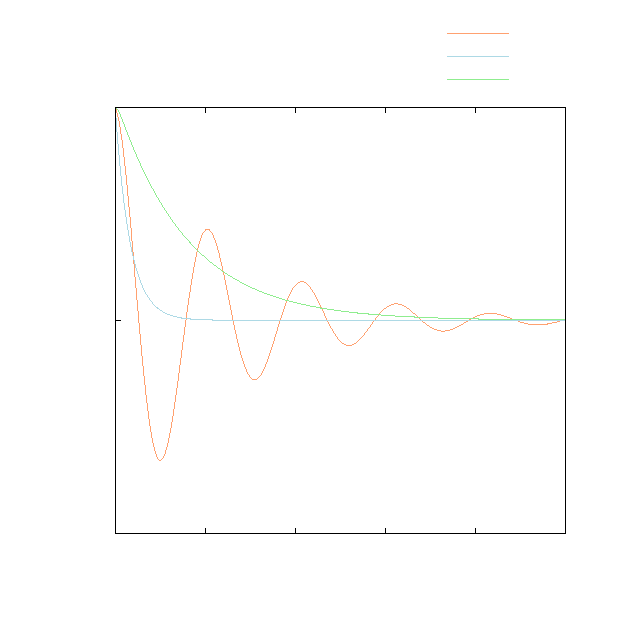
\includegraphics{oscilacions}}%
    \gplfronttext
  \end{picture}%
\endgroup

	\caption{Representació del voltatge al condensador en tres règims d'amortiment diferents}
	\label{fig:oscilacions}
\end{figure}

\section{Conclusions}
\subsection{Règim transitori}

